Los drones Crazyflie han demostrado ser herramientas altamente efectivas en investigación de sistemas de control, ya sea como agentes individuales o dentro de un enjambre. Algunos ejemplos de investigación incluyen estudios sobre algoritmos de evasión de obstáculos, vuelo en enjambre y sistemas de navegación autónoma. Esta eficacia y versatilidad de los drones fue la razón principal por la cual la Universidad del Valle de Guatemala adquirió hace algunos años un conjunto de drones Crazyflie y, desde entonces, se han desarrollado diversos proyectos de investigación con ellos.

\section{Investigación con drones Crazyflie en la Universidad del Valle de Guatemala}
Sanabria en \cite{Sanabria2022_tesis} desarrolló la fase inicial en la línea de investigación con drones Crazyflie. Su trabajo consistió en la implementación de una plataforma de pruebas \ref{fig:Sanabria2022} para cuadricópteros Crazyflie 2.0 sobre la cual se pueden verificar algoritmos de control de actitud para un grado de libertad. Durante su investigación, implementó un conjunto de herramientas de \textit{software} necesarias para comunicar al dron con la computadora a través de Python y por medio del dispositivo Crazyradio. Asimismo, elaboró una interfaz gráfica capaz de recuperar y procesar ángulos de inclinación, manipular la orientación y modificar los parámetros del controlador del dron. 

\begin{figure}[htbp]
	\centering
	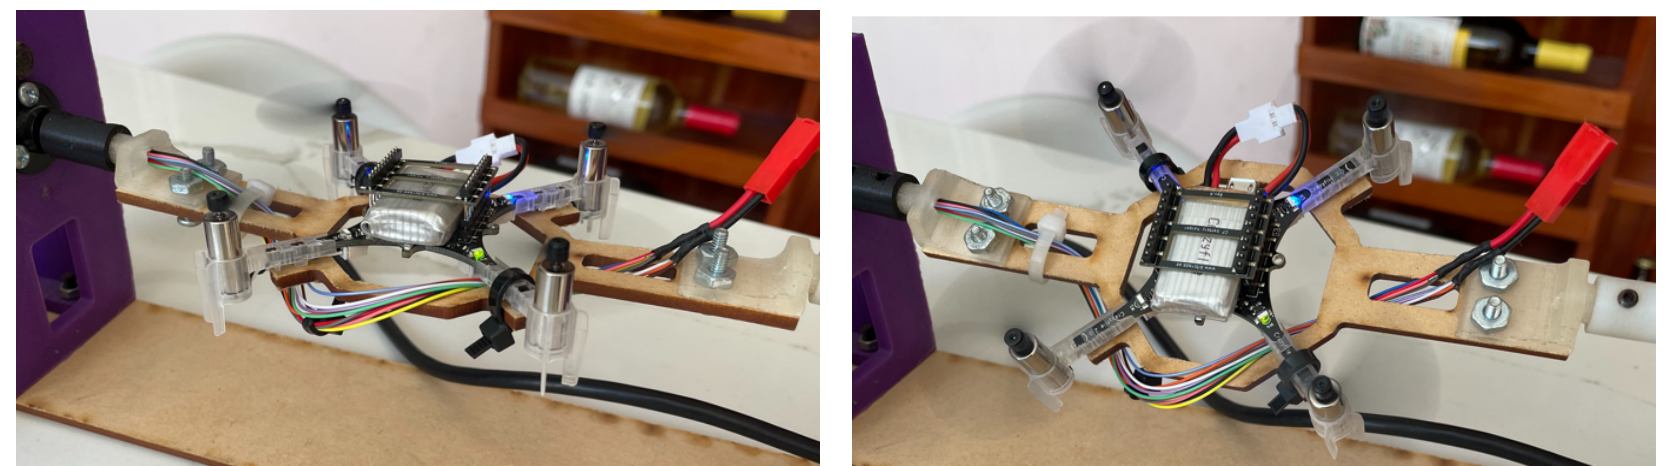
\includegraphics[width=0.75\textwidth]{Sanabria2022}
	\caption{Plataforma de pruebas de la investigación de Sanabria \cite{Sanabria2022_tesis}.}
	\label{fig:Sanabria2022}
\end{figure}

Como resultado de la investigación se crearon guías de laboratorio para los cursos de sistemas de control 1 y 2, con la limitante de que el dron únicamente podría utilizarse junto a la plataforma de pruebas.

\section{Ecosistema Robotat}
El ecosistema Robotat \ref{fig:Robotat} es un entrono tecnológico de investigación y experimentación ubicado en la Universidad del Valle de Guatemala \cite{Parafan2022_tesis}. Este ecosistema consiste de una plataforma sólida de aproximadamente $400\times 500$ cm, un sistema de captura de movimiento compuesto por seis cámaras OptiTrack y una red local Wi-Fi estblecida mediante el protocolo MQTT. La infraestructura permite la conexión y control de múltiples agentes simultáneamente, con una capacidad máxima de 11 agentes operando a una frecuencia de recepción y decodificación de datos superior a 10 Hz. 

\vspace{0.3cm} % Espacio antes de la imagen
\begin{figure}[htbp]
	\centering
	\includegraphics[width=0.75\textwidth]{Robotat}
	\caption{Ecosistema de pruebas Robotat \cite{Parafan2022_tesis}.}
	\label{fig:Robotat}
\end{figure}

\section{Incorporación de drones Crazyflie al ecosistema Robotat}
Denny Otzoy \cite{Otzoy2023_tesis} y José Gordillo \cite{Gordillo2023_tesis} se centraron en desarrollar la infraestructura y herramientas necesarias para utilizar el cuadricóptero dentro del ecosistema Robotat. Otzoy se enfocó en el desarrollo de herramientas para la integración con el sistema de captura de movimiento. Empleó una máquina física para la transmisión de datos, desarrolló la representación del dron como cuerpo rígido dentro del ecosistema y codificó las trayectorias en el formato adecuado. Por otro lado, Gordillo implementó un paquete de herramientas de \textit{software} para la ejecución de trayectorias de enjambre. Evaluó dos alternativas para el sistema de control y con base en un listado de ventajas y desventajas, descartó la opción de la librería Crazyswarm y en su lugar optó por implementar un sistema basado en una antena de comunicación WiFi. En ambos casos, a pesar de los esfuerzos, no se logró el control adecuado o seguimiento de trayectorias debido a limitantes en la metodología empleada para el sistema de control del dron. 

A raíz de las limitaciones encontradas, Julio Avila \cite{Avila2023_tesis} y Brandon Garrido \cite{Garrido2023_tesis} buscaron integrar la librería de control Crazyswarm 2 al ecosistema Robotat. El trabajo de Avila estuvo centrado principalmente en el desarrollo de un servidor para comunicación entre los drones, el sistema de captura de movimiento y Matlab, con el fin de enviar comandos para realizar trayectorias de drones individuales o de enjambre. Por su parte, Garrido se enfocó en el desarrollo de infraestructura para la experimentación y control de múltiples drones desde el sistema operativo ROS2 y dentro del ecosistema Robotat. Los resultados obtenidos en ambas investigaciones demostraron estabilidad y precisión en el control de los drones. 

\vspace{0.5cm} % Espacio antes de la imagen
\begin{figure}[htbp]
	\centering
	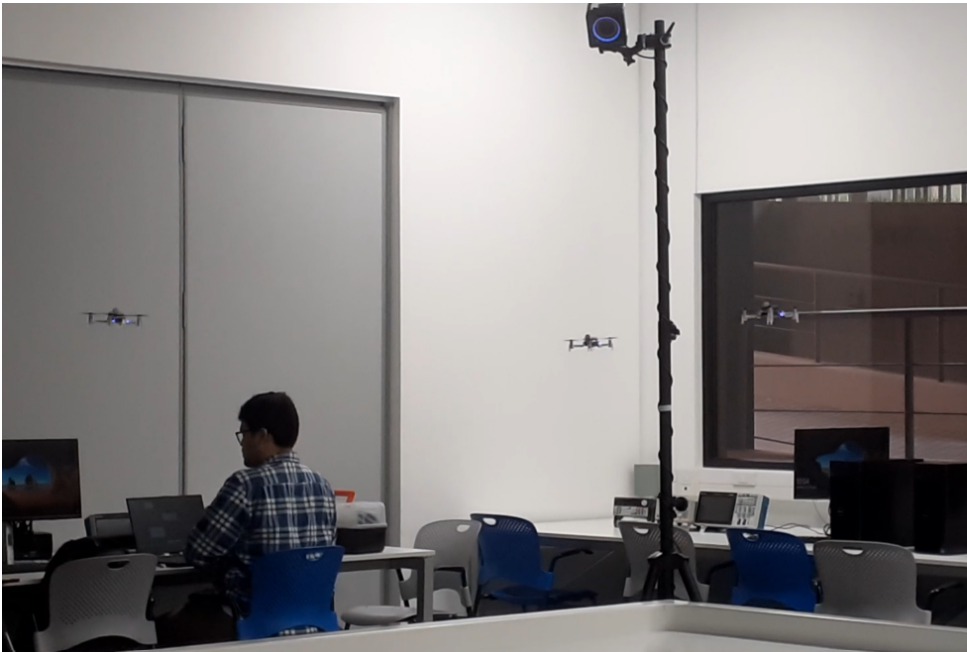
\includegraphics[width=0.75\textwidth]{Crazyswarm}
	\caption{Prueba de vuelo con 3 drones utilizando el \textit{software} Crazyswarm 2 \cite{Garrido2023_tesis}.}
	\label{fig:Crazyswarm}
\end{figure}
\vspace{0.4cm} % Espacio después de la imagen

Aunque el manejo de los drones mediante Crazyswarm demostró ser efectivo, requiere conocimientos de los sistemas operativos Linux y ROS2. Esta tarea vuelve complicado el proceso debido a la complejidad de dichas herramientas y la escasa documentación disponible de la librería Crazyswarm 2. Adicionalmente, la transición de Crazyflie a ROS2 es reciente, al igual que la librería Crazyswarm 2, lo que dificulta su implementación en laboratorios. 

Por otro lado, el uso individual de los drones Crazyflie plantea otro desafío, ya que, sin un medio para conocer su posición, los drones son vulnerables a colisiones debido a la fragilidad de su manipulación. Para abordar dicho desafío, una solución viable es complementar el funcionamiento de los drones con alguna de las placas de expansión de Bitcraze. Una de ellas es el Flow Deck, que ha demostrado ser altamente eficiente en proporcionar estabilidad al dron y con el cual se han logrado proyectos de investigación como vuelo autónomo y seguimiento de trayectorias.

\newpage
\section{Vuelo autónomo del dron Crazyflie 2.1 empleando la placa de posicionamiento Flow Deck}
En la Universidad Uppsala \cite{Chadehumbe2020_tesis} se realizó una investigación utilizando drones Crazyflie 2.1 con el objetivo de incorporar vuelo autónomo a través de trayectorias con obstáculos. Para ello se exploraron dos alternativas para el sistema de navegación del dron: un sistema de posicionamiento local mediante la herramienta LPS (\textit{Loco Positioning System}) y un sistema de navegación óptico mediante el dispositivo Flow Deck. Para la detección de obstáculos en las trayectorias se utilizó el sensor de detección Multiranger. 

Durante los experimentos realizados se observó que el sistema de navegación óptico superó al LPS en términos de estabilidad de vuelo y capacidad para completar las trayectorias. No se logró completar pruebas realizadas con el LPS como sistema de posicionamiento, siendo la razón principal el vuelo inestable causado por perturbaciones inusuales en el entorno de experimentación. Por otro lado, se completaron satisfactoriamente las pruebas al emplear el sistema de navegación óptico con el Flow Deck. Como recomendación, se sugirió realizar pruebas adicionales para mejorar la precisión del vuelo y considerar la posibilidad de utilizar múltiples sistemas de navegación en conjunto para obtener resultados más robustos.